

\tikzset{every picture/.style={line width=0.75pt}} %set default line width to 0.75pt        

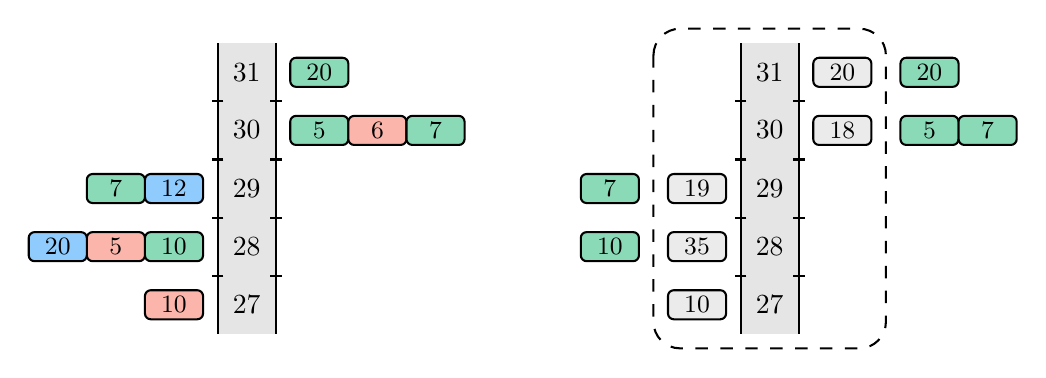
\begin{tikzpicture}[x=0.75pt,y=0.75pt,yscale=-0.7,xscale=0.7]
%uncomment if require: \path (0,300); %set diagram left start at 0, and has height of 300


%Shape: Rectangle [id:dp5489135505501248] 
\draw  [draw opacity=0][fill={rgb, 255:red, 0; green, 0; blue, 0 }  ,fill opacity=0.1 ] (140,60) -- (180,60) -- (180,260) -- (140,260) -- cycle ;
%Rounded Rect [id:dp5571720629473116] 
\draw  [fill={rgb, 255:red, 138; green, 218; blue, 184 }  ,fill opacity=1 ][line width=0.75]  (190,114) .. controls (190,111.79) and (191.79,110) .. (194,110) -- (226,110) .. controls (228.21,110) and (230,111.79) .. (230,114) -- (230,126) .. controls (230,128.21) and (228.21,130) .. (226,130) -- (194,130) .. controls (191.79,130) and (190,128.21) .. (190,126) -- cycle ;
%Straight Lines [id:da6082688802942293] 
\draw    (140,60) -- (140,260) (144,100) -- (136,100)(144,140) -- (136,140)(144,180) -- (136,180)(144,220) -- (136,220) ;
%Straight Lines [id:da9720053745263018] 
\draw    (180,60) -- (180,260) (184,100) -- (176,100)(184,140) -- (176,140)(184,180) -- (176,180)(184,220) -- (176,220) ;
%Rounded Rect [id:dp10362529279551769] 
\draw  [fill={rgb, 255:red, 251; green, 181; blue, 170 }  ,fill opacity=1 ][line width=0.75]  (230,114) .. controls (230,111.79) and (231.79,110) .. (234,110) -- (266,110) .. controls (268.21,110) and (270,111.79) .. (270,114) -- (270,126) .. controls (270,128.21) and (268.21,130) .. (266,130) -- (234,130) .. controls (231.79,130) and (230,128.21) .. (230,126) -- cycle ;
%Rounded Rect [id:dp3209795107013548] 
\draw  [fill={rgb, 255:red, 138; green, 218; blue, 184 }  ,fill opacity=1 ][line width=0.75]  (270,114) .. controls (270,111.79) and (271.79,110) .. (274,110) -- (306,110) .. controls (308.21,110) and (310,111.79) .. (310,114) -- (310,126) .. controls (310,128.21) and (308.21,130) .. (306,130) -- (274,130) .. controls (271.79,130) and (270,128.21) .. (270,126) -- cycle ;
%Rounded Rect [id:dp14006433626528436] 
\draw  [fill={rgb, 255:red, 138; green, 218; blue, 184 }  ,fill opacity=1 ][line width=0.75]  (190,74) .. controls (190,71.79) and (191.79,70) .. (194,70) -- (226,70) .. controls (228.21,70) and (230,71.79) .. (230,74) -- (230,86) .. controls (230,88.21) and (228.21,90) .. (226,90) -- (194,90) .. controls (191.79,90) and (190,88.21) .. (190,86) -- cycle ;
%Rounded Rect [id:dp23032489064391803] 
\draw  [fill={rgb, 255:red, 138; green, 218; blue, 184 }  ,fill opacity=1 ][line width=0.75]  (90,194) .. controls (90,191.79) and (91.79,190) .. (94,190) -- (126,190) .. controls (128.21,190) and (130,191.79) .. (130,194) -- (130,206) .. controls (130,208.21) and (128.21,210) .. (126,210) -- (94,210) .. controls (91.79,210) and (90,208.21) .. (90,206) -- cycle ;
%Rounded Rect [id:dp2906178876656058] 
\draw  [fill={rgb, 255:red, 143; green, 203; blue, 253 }  ,fill opacity=1 ][line width=0.75]  (90,154) .. controls (90,151.79) and (91.79,150) .. (94,150) -- (126,150) .. controls (128.21,150) and (130,151.79) .. (130,154) -- (130,166) .. controls (130,168.21) and (128.21,170) .. (126,170) -- (94,170) .. controls (91.79,170) and (90,168.21) .. (90,166) -- cycle ;
%Rounded Rect [id:dp2773205270553206] 
\draw  [fill={rgb, 255:red, 138; green, 218; blue, 184 }  ,fill opacity=1 ][line width=0.75]  (50,154) .. controls (50,151.79) and (51.79,150) .. (54,150) -- (86,150) .. controls (88.21,150) and (90,151.79) .. (90,154) -- (90,166) .. controls (90,168.21) and (88.21,170) .. (86,170) -- (54,170) .. controls (51.79,170) and (50,168.21) .. (50,166) -- cycle ;
%Rounded Rect [id:dp4559050638577514] 
\draw  [fill={rgb, 255:red, 251; green, 181; blue, 170 }  ,fill opacity=1 ][line width=0.75]  (50,194) .. controls (50,191.79) and (51.79,190) .. (54,190) -- (86,190) .. controls (88.21,190) and (90,191.79) .. (90,194) -- (90,206) .. controls (90,208.21) and (88.21,210) .. (86,210) -- (54,210) .. controls (51.79,210) and (50,208.21) .. (50,206) -- cycle ;
%Rounded Rect [id:dp12376095296435441] 
\draw  [fill={rgb, 255:red, 143; green, 203; blue, 253 }  ,fill opacity=1 ][line width=0.75]  (10,194) .. controls (10,191.79) and (11.79,190) .. (14,190) -- (46,190) .. controls (48.21,190) and (50,191.79) .. (50,194) -- (50,206) .. controls (50,208.21) and (48.21,210) .. (46,210) -- (14,210) .. controls (11.79,210) and (10,208.21) .. (10,206) -- cycle ;
%Rounded Rect [id:dp5644180007175256] 
\draw  [fill={rgb, 255:red, 251; green, 181; blue, 170 }  ,fill opacity=1 ][line width=0.75]  (90,234) .. controls (90,231.79) and (91.79,230) .. (94,230) -- (126,230) .. controls (128.21,230) and (130,231.79) .. (130,234) -- (130,246) .. controls (130,248.21) and (128.21,250) .. (126,250) -- (94,250) .. controls (91.79,250) and (90,248.21) .. (90,246) -- cycle ;
%Shape: Rectangle [id:dp5662774353889877] 
\draw  [draw opacity=0][fill={rgb, 255:red, 0; green, 0; blue, 0 }  ,fill opacity=0.1 ] (500,60) -- (540,60) -- (540,260) -- (500,260) -- cycle ;
%Rounded Rect [id:dp08118930746789832] 
\draw  [fill={rgb, 255:red, 235; green, 235; blue, 235 }  ,fill opacity=1 ][line width=0.75]  (550,114) .. controls (550,111.79) and (551.79,110) .. (554,110) -- (586,110) .. controls (588.21,110) and (590,111.79) .. (590,114) -- (590,126) .. controls (590,128.21) and (588.21,130) .. (586,130) -- (554,130) .. controls (551.79,130) and (550,128.21) .. (550,126) -- cycle ;
%Straight Lines [id:da20677085553463082] 
\draw    (500,60) -- (500,260) (504,100) -- (496,100)(504,140) -- (496,140)(504,180) -- (496,180)(504,220) -- (496,220) ;
%Straight Lines [id:da40710486463167805] 
\draw    (540,60) -- (540,260) (544,100) -- (536,100)(544,140) -- (536,140)(544,180) -- (536,180)(544,220) -- (536,220) ;
%Rounded Rect [id:dp6364145985594639] 
\draw  [fill={rgb, 255:red, 235; green, 235; blue, 235 }  ,fill opacity=1 ][line width=0.75]  (550,74) .. controls (550,71.79) and (551.79,70) .. (554,70) -- (586,70) .. controls (588.21,70) and (590,71.79) .. (590,74) -- (590,86) .. controls (590,88.21) and (588.21,90) .. (586,90) -- (554,90) .. controls (551.79,90) and (550,88.21) .. (550,86) -- cycle ;
%Rounded Rect [id:dp2804611471386602] 
\draw  [fill={rgb, 255:red, 235; green, 235; blue, 235 }  ,fill opacity=1 ][line width=0.75]  (450,194) .. controls (450,191.79) and (451.79,190) .. (454,190) -- (486,190) .. controls (488.21,190) and (490,191.79) .. (490,194) -- (490,206) .. controls (490,208.21) and (488.21,210) .. (486,210) -- (454,210) .. controls (451.79,210) and (450,208.21) .. (450,206) -- cycle ;
%Rounded Rect [id:dp24217444343409034] 
\draw  [fill={rgb, 255:red, 235; green, 235; blue, 235 }  ,fill opacity=1 ][line width=0.75]  (450,154) .. controls (450,151.79) and (451.79,150) .. (454,150) -- (486,150) .. controls (488.21,150) and (490,151.79) .. (490,154) -- (490,166) .. controls (490,168.21) and (488.21,170) .. (486,170) -- (454,170) .. controls (451.79,170) and (450,168.21) .. (450,166) -- cycle ;
%Rounded Rect [id:dp045526064729431215] 
\draw  [fill={rgb, 255:red, 235; green, 235; blue, 235 }  ,fill opacity=1 ][line width=0.75]  (450,234) .. controls (450,231.79) and (451.79,230) .. (454,230) -- (486,230) .. controls (488.21,230) and (490,231.79) .. (490,234) -- (490,246) .. controls (490,248.21) and (488.21,250) .. (486,250) -- (454,250) .. controls (451.79,250) and (450,248.21) .. (450,246) -- cycle ;
%Rounded Rect [id:dp6633295562595507] 
\draw  [fill={rgb, 255:red, 138; green, 218; blue, 184 }  ,fill opacity=1 ][line width=0.75]  (390,194) .. controls (390,191.79) and (391.79,190) .. (394,190) -- (426,190) .. controls (428.21,190) and (430,191.79) .. (430,194) -- (430,206) .. controls (430,208.21) and (428.21,210) .. (426,210) -- (394,210) .. controls (391.79,210) and (390,208.21) .. (390,206) -- cycle ;
%Rounded Rect [id:dp641336334884714] 
\draw  [fill={rgb, 255:red, 138; green, 218; blue, 184 }  ,fill opacity=1 ][line width=0.75]  (390,154) .. controls (390,151.79) and (391.79,150) .. (394,150) -- (426,150) .. controls (428.21,150) and (430,151.79) .. (430,154) -- (430,166) .. controls (430,168.21) and (428.21,170) .. (426,170) -- (394,170) .. controls (391.79,170) and (390,168.21) .. (390,166) -- cycle ;
%Rounded Rect [id:dp4238339096677155] 
\draw  [fill={rgb, 255:red, 138; green, 218; blue, 184 }  ,fill opacity=1 ][line width=0.75]  (610,114) .. controls (610,111.79) and (611.79,110) .. (614,110) -- (646,110) .. controls (648.21,110) and (650,111.79) .. (650,114) -- (650,126) .. controls (650,128.21) and (648.21,130) .. (646,130) -- (614,130) .. controls (611.79,130) and (610,128.21) .. (610,126) -- cycle ;
%Rounded Rect [id:dp3352222243665929] 
\draw  [fill={rgb, 255:red, 138; green, 218; blue, 184 }  ,fill opacity=1 ][line width=0.75]  (650,114) .. controls (650,111.79) and (651.79,110) .. (654,110) -- (686,110) .. controls (688.21,110) and (690,111.79) .. (690,114) -- (690,126) .. controls (690,128.21) and (688.21,130) .. (686,130) -- (654,130) .. controls (651.79,130) and (650,128.21) .. (650,126) -- cycle ;
%Rounded Rect [id:dp018044766031021897] 
\draw  [fill={rgb, 255:red, 138; green, 218; blue, 184 }  ,fill opacity=1 ][line width=0.75]  (610,74) .. controls (610,71.79) and (611.79,70) .. (614,70) -- (646,70) .. controls (648.21,70) and (650,71.79) .. (650,74) -- (650,86) .. controls (650,88.21) and (648.21,90) .. (646,90) -- (614,90) .. controls (611.79,90) and (610,88.21) .. (610,86) -- cycle ;
%Rounded Rect [id:dp43481833872293096] 
\draw  [dash pattern={on 4.5pt off 4.5pt}] (440,68.3) .. controls (440,58.19) and (448.19,50) .. (458.3,50) -- (581.7,50) .. controls (591.81,50) and (600,58.19) .. (600,68.3) -- (600,251.7) .. controls (600,261.81) and (591.81,270) .. (581.7,270) -- (458.3,270) .. controls (448.19,270) and (440,261.81) .. (440,251.7) -- cycle ;

% Text Node
\draw (160,80) node    {$31$};
% Text Node
\draw (160,119.5) node    {$30$};
% Text Node
\draw (210,120) node  [font=\small]  {${\textstyle 5}$};
% Text Node
\draw (160,160) node    {$29$};
% Text Node
\draw (160,200) node    {$28$};
% Text Node
\draw (160,240) node    {$27$};
% Text Node
\draw (250,120) node  [font=\small]  {$6$};
% Text Node
\draw (290,120) node  [font=\small]  {$7$};
% Text Node
\draw (210,80) node  [font=\small]  {$20$};
% Text Node
\draw (110,200) node  [font=\small]  {$10$};
% Text Node
\draw (110,160) node  [font=\small]  {$12$};
% Text Node
\draw (70,160) node  [font=\small]  {$7$};
% Text Node
\draw (70,200) node  [font=\small]  {${\textstyle 5}$};
% Text Node
\draw (30,200) node  [font=\small]  {$20$};
% Text Node
\draw (110,240) node  [font=\small]  {$10$};
% Text Node
\draw (520,80) node    {$31$};
% Text Node
\draw (520,119.5) node    {$30$};
% Text Node
\draw (570,120) node  [font=\small]  {$18$};
% Text Node
\draw (520,160) node    {$29$};
% Text Node
\draw (520,200) node    {$28$};
% Text Node
\draw (520,240) node    {$27$};
% Text Node
\draw (570,80) node  [font=\small]  {$20$};
% Text Node
\draw (470,200) node  [font=\small]  {$35$};
% Text Node
\draw (470,160) node  [font=\small]  {$19$};
% Text Node
\draw (470,240) node  [font=\small]  {$10$};
% Text Node
\draw (410,200) node  [font=\small]  {$10$};
% Text Node
\draw (410,160) node  [font=\small]  {$7$};
% Text Node
\draw (630,120) node  [font=\small]  {$5$};
% Text Node
\draw (670,120) node  [font=\small]  {$7$};
% Text Node
\draw (630,80) node  [font=\small]  {$20$};


\end{tikzpicture}
